% statistics_and_probability:x04 GDC:NO
\begin{question}
  \hspace*{\fill} [Note maximale: 8]\par
  \medskip
  \noindent La variable aléatoire X suit la distribution de probabilité suivante, avec P(X >1) = 0,5.\par

  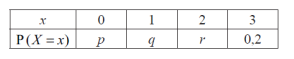
\includegraphics[scale=0.7]{px_table}  

  (a) Trouvez la valeur de r.\hspace*{\fill} [2]\par
  (b) Étant donné que E(X ) =1,4 , trouvez la valeur de p et celle de q. \hspace*{\fill} [6]\par
  
\end{question}

